\documentclass{book}

\usepackage{fullpage}

%\usepackage{wrapfig}
%\usepackage{float}
%  \floatstyle{ruled}
%  \newfloat{callout}{thp}{lop}
%  \floatname{callout}{Things To Remember}

\usepackage{color}
\definecolor{Light}{gray}{.95}

\usepackage{amsthm}
{
  \theoremstyle{definition}
  \newtheorem{example}{Example}
}

\usepackage{graphicx}

\newlength{\calloutparindent}
\setlength{\calloutparindent}{\parindent}
%%
%% begin: the callout command
\newcommand{\callout}[3]{\label{#1}\vspace{3mm}
\begin{center}
\fcolorbox{black}{Light}{\begin{minipage}{0.85\textwidth}
    \textbf{\large Things To Remember~\ref{#1} --- #2}
    \hrule
    \vspace{2mm}
\setlength{\parindent}{\calloutparindent}
#3
  \end{minipage}}
\end{center}
\vspace{3mm}
}
\newcommand{\thingstoremember}[1]{Things To Remember~\ref{#1}}
%% end: the callout command
%%

% two chapters will precede the one here now
\setcounter{chapter}{3}

\begin{document}

\chapter{Delegation}

An important design decision when modeling data is how many Java classes to use to represent an entity. At one extreme, all of the attributes of an entity are represented by a single class, resulting in a coarse-grained design. At the other extreme, a main entity class delegates functionality to other classes, resulting in a fine-grained design.  Delegation is a very popular pattern because of the flexibility it provides. 

Programmers rarely think about memory costs when deciding how to model entities. Yet, the choices made at this design stage impact memory costs significantly. Coarse-grained designs may result in many objects with unused fields. While delegation is sometimes a way to avoid this problem, overly fine-grained data models can result in poor memory health from excessive object header overhead. This chapter explains how to evaluate object granularity design choices from a memory perspective. It begins with the costs of basic objects, and works up to examples from real applications.
  
\section{The Cost of Objects}
\label{sec:CostOfObjects}

There is no Java library method that returns the size of an object. This is by design. A Java programmer is not supposed to know either the size of an object or how it is layed out in memory. But if you know the costs of the built in primitives and types, it is not hard to compute a reasonable estimate. (You can obtain the exact size of objects by running your program the HPROF agent.)  

Java specifies the sizes needed to store primitive types:
\begin{table}
  \centering
 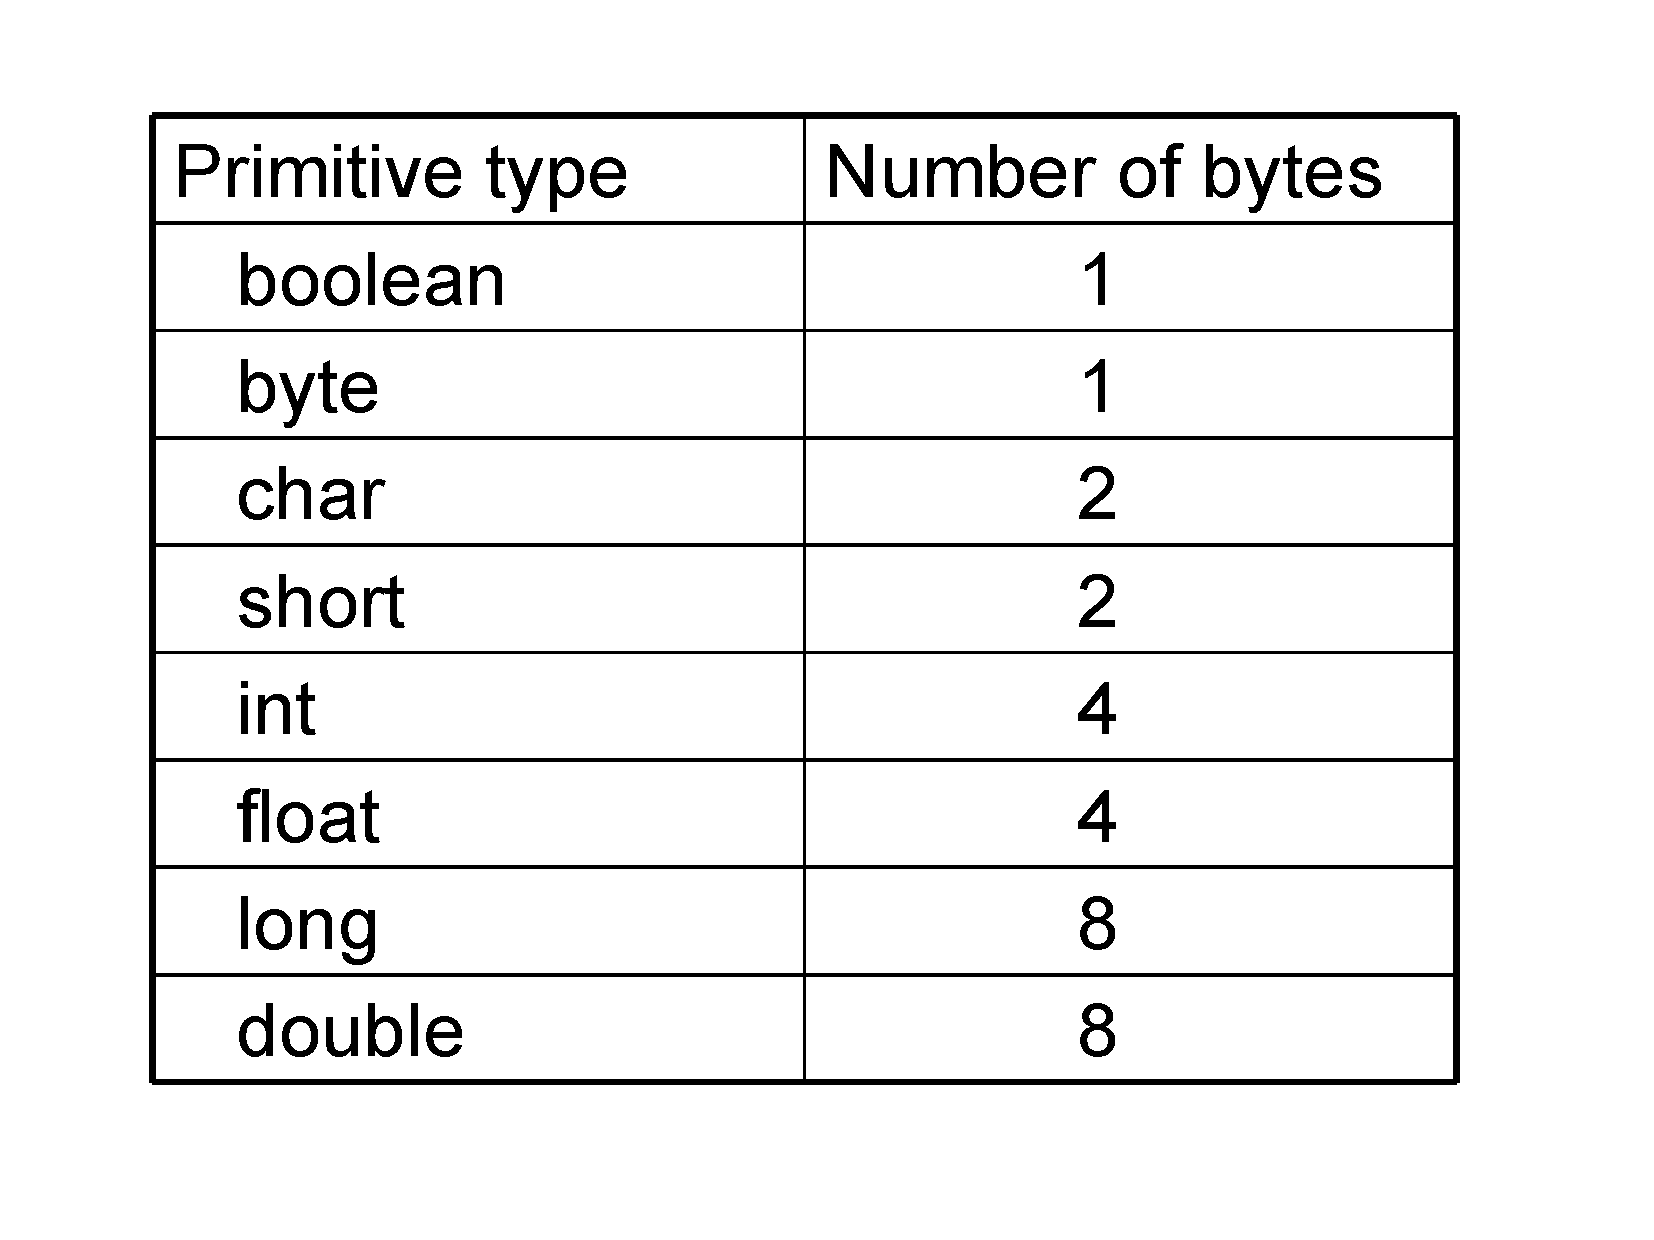
\includegraphics[width=.40\textwidth]{Figures/chapter4/primitive-byte-sizes.pdf}
 % 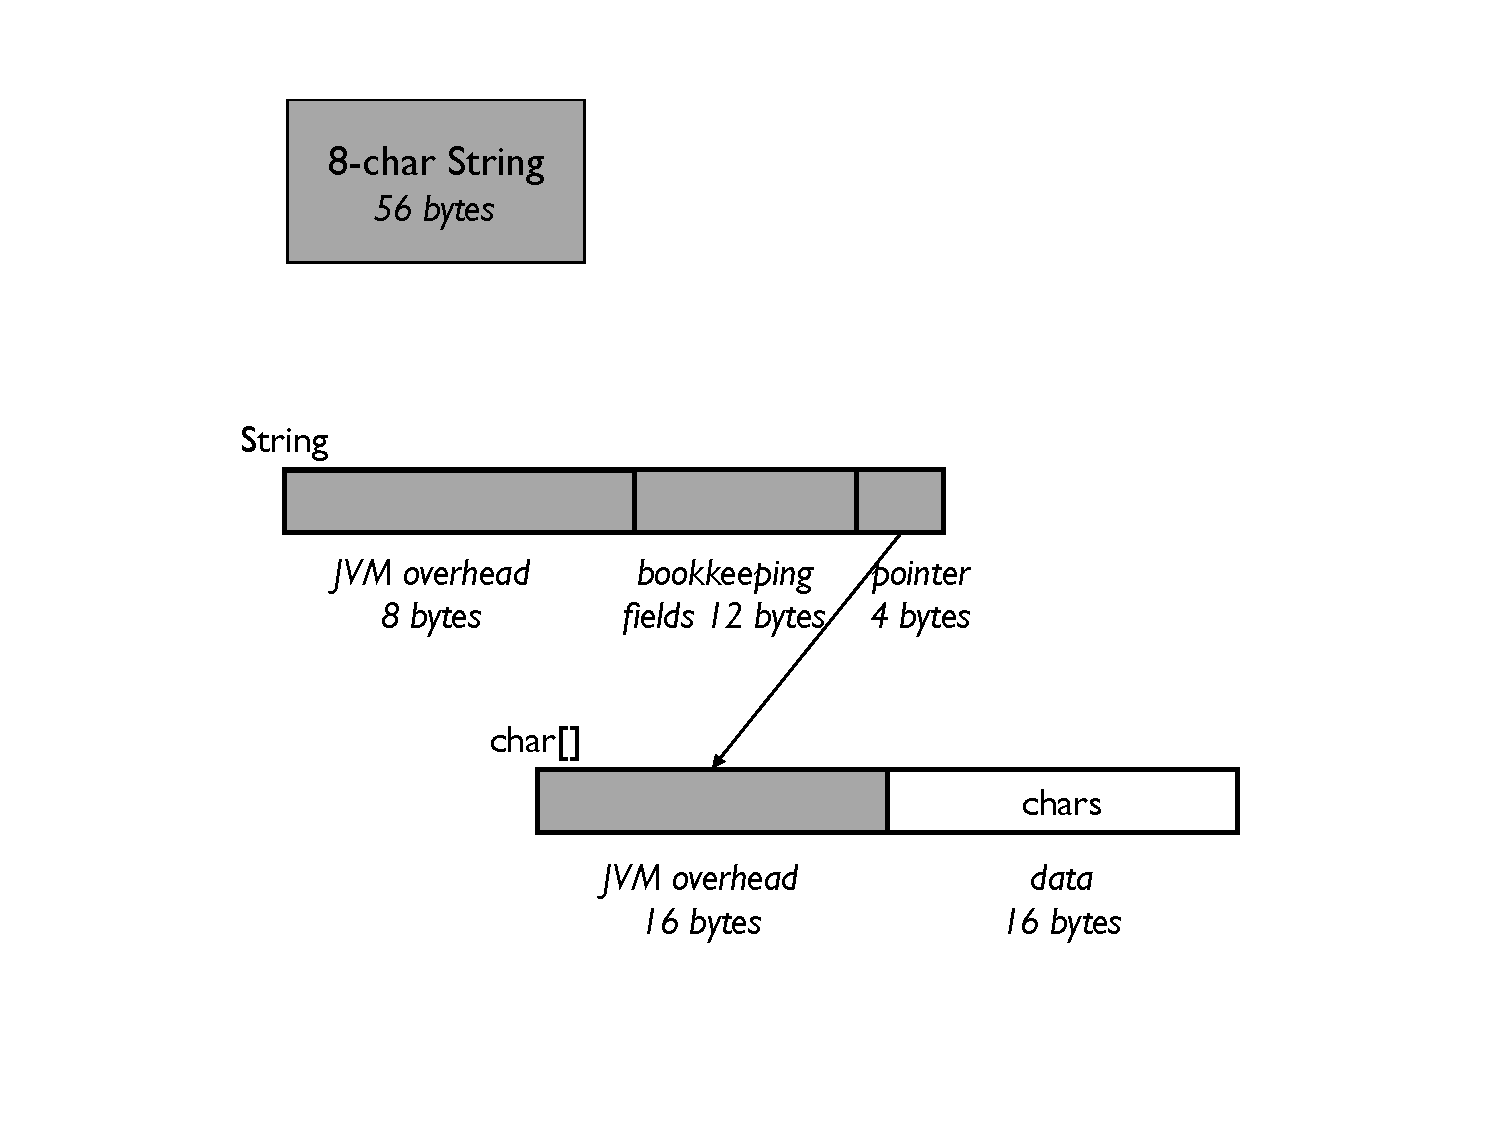
\includegraphics{eight-char-string}
  \caption{The sizes of Java primitive types}
  \label{tab:primitive-sizes}
\end{table}

Objects are much bigger. Both the JVM and the hardware impose costs, which are substantial for small objects. These costs can differ, depending on the JVM and on the hardware.  Each object has a header that stores information that the JVM and garbage collector needs, such as the class, an active monitor and an identity hashcode. 

The underlying hardware can impose alignment costs. The hardware may require 2-byte, 4-byte, or 8-byte alignment, depending on the type of the data. For example, integers are usually aligned on a 4-byte boundary, and some hardware might require a double to be aligned on an 8-byte boundary. A JVM may impose an alignment requirement above and beyond the hardware, if there is some performance benefits for storage allocation and garbage collection. 

The numbers given here are for both the SUN Java 6u1.4 JVM and the IBM J9SR4 JVM on 32-bit architectures. These numbers may change in future JVM releases, but are useful to give concrete examples.
   
The Sun Java 6u1.4 JVM allocates 8 bytes per object header, and the IBM J9SR4 JVM allocates 12 bytes per header. For array objects, the header has an additional integer to store the number of array elements. The array header size increases to 12 bytes for Sun 6u1.4, and 16 bytes for J9SR4. 

Both JVMs allocate objects on 8-byte boundaries. This means that the size of an object is a multiple of 8. For both JVMs, the smallest that an object with at least one byte of data can be is 16 bytes. 

The table~\ref{tab:boxed-scalar-sizes} gives the sizes for boxed scalars.

\begin{table}
  \centering
 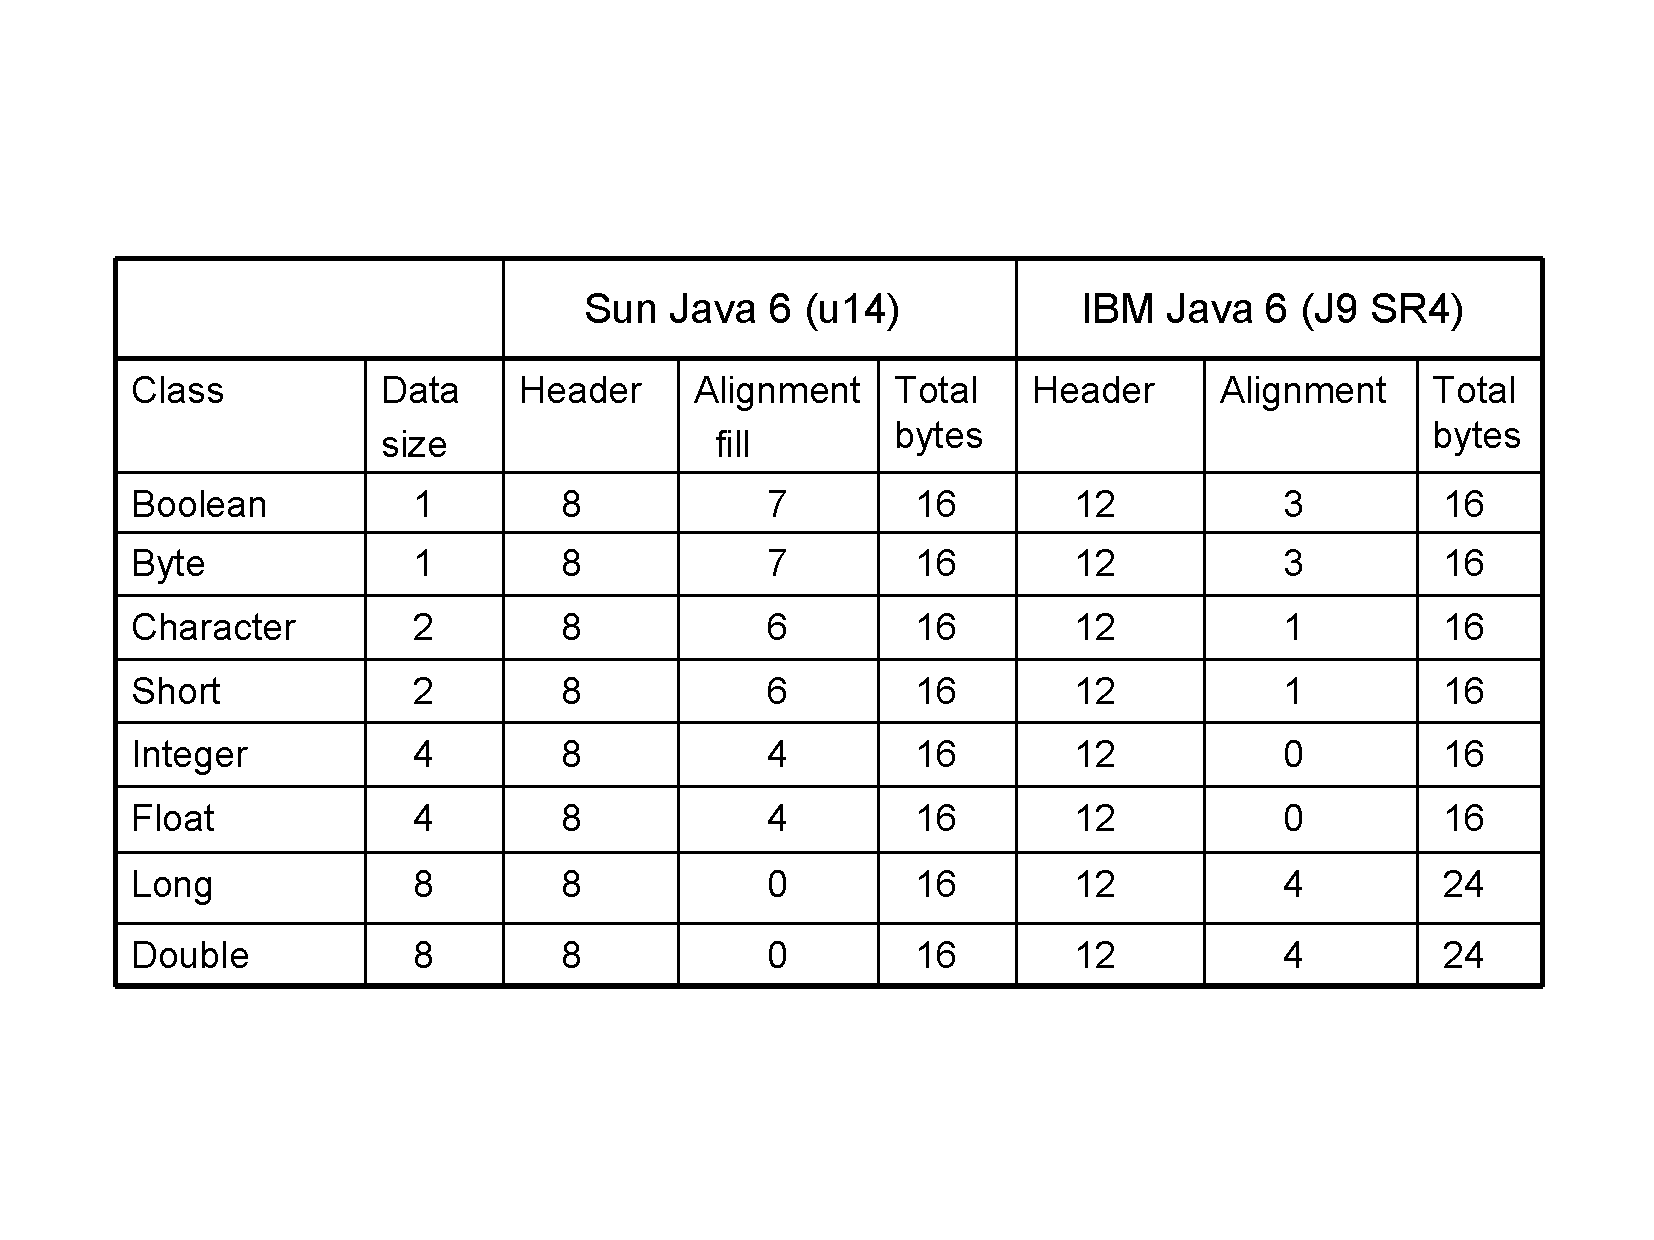
\includegraphics[width=.60\textwidth]{Figures/chapter4/boxed-scalar-sizes.pdf}
 % 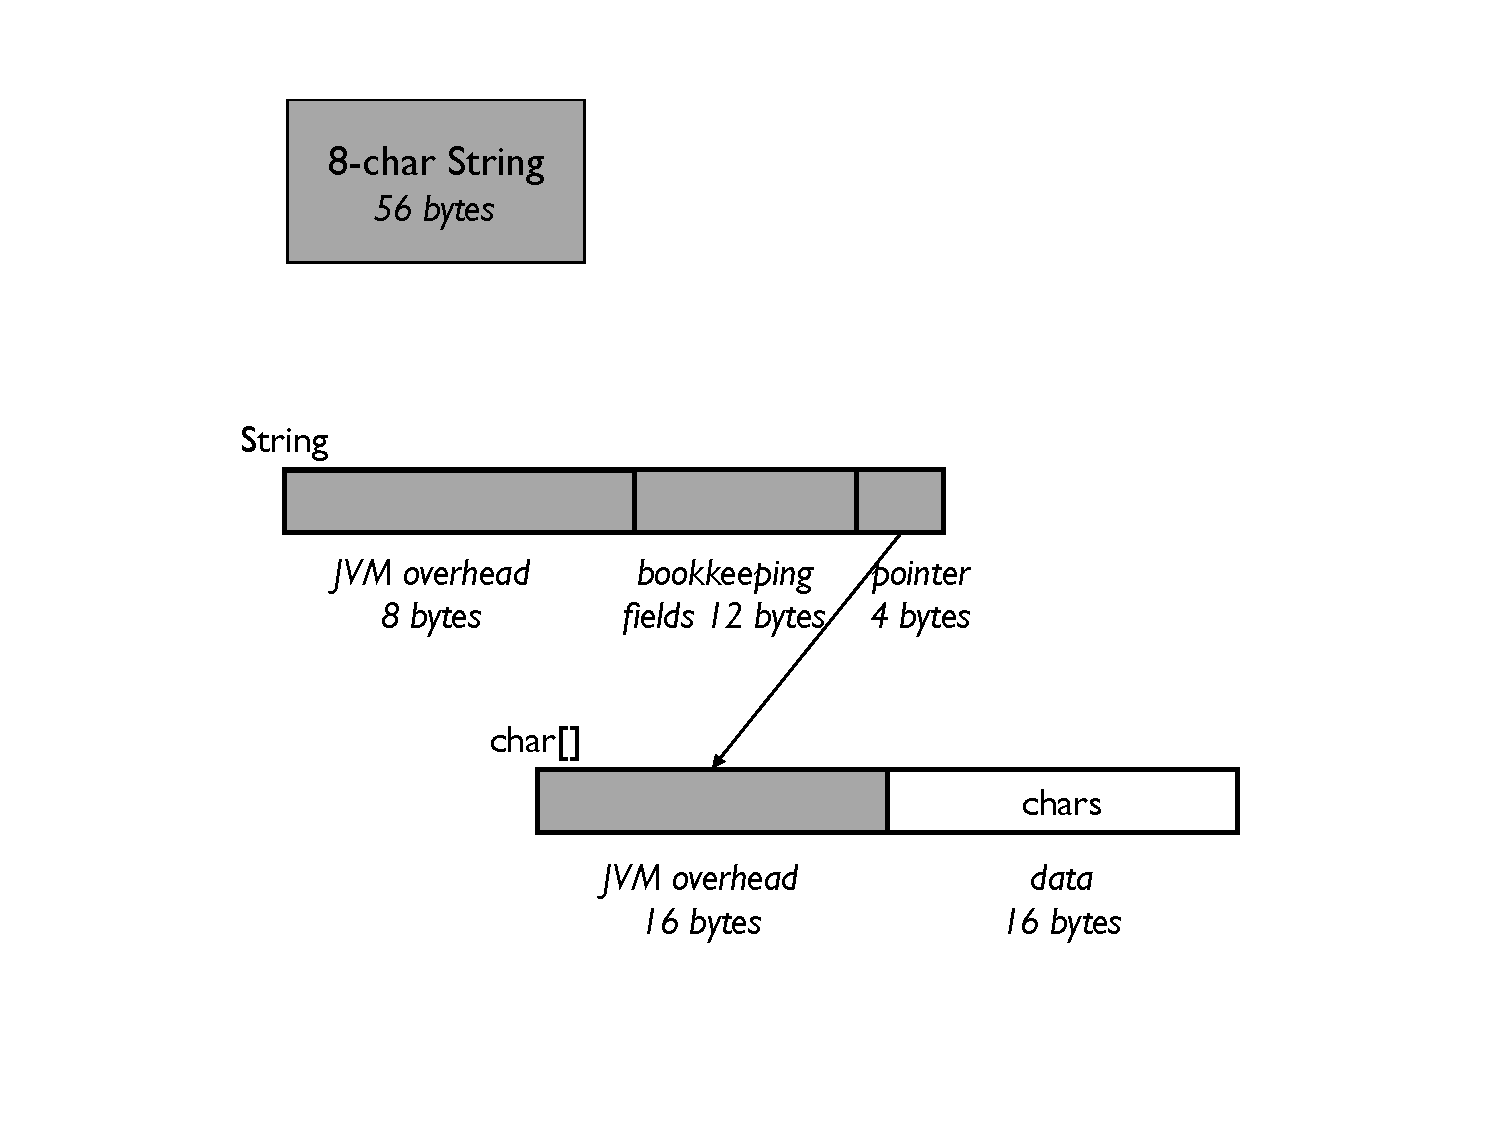
\includegraphics{eight-char-string}
  \caption{The sizes of boxed scalar objects.}
  \label{tab:boxed-scalar-sizes}
\end{table} 

There is a simple rule that holds here. The size of the object is obtained by adding together the size of the header and the data, and then rounding it up to the nearest multiple of 8. The generalization of this rule gives you a good way to estimate the size of any object. Often, this estimate turns out to be the real object size, but not always. The JVM has freedom in the way it lays out an object. 
 
\callout{callout:object-size-estimation-rule}{Minimum Size Estimation Rule}{
    Let $Header$ be the size of an object header required by the JVM, and $Alignment$ be the object alignment. That is, every object must be allocated at an address which is a multiple of $Alignment$. You can estimate the size of an object by 1) summing up the sizes of all of the data stored in the object, including data from superclasses, 2) adding this sum to $Header$, and 3) rounding the result up to the next multiple of $Alignment$. 
    
	This rule computes the minimum size of an object. The calculation is exact if the JVM packs and rearranges fields to fit into the smallest space.
}


\begin{example}[Employee class and subclass.]
Consider an \texttt{EmployeeStatus} class with all primitive fields:

\ttfamily
\begin{verbatim} 

			class EmployeeStatus {
        int hoursPerWeek;
        boolean exempt;
        double salary;
        char jobCode;
        int yearsOfService;
			}
\end{verbatim}
\normalfont
Applying the object size estimation rule, assuming both $Header$ and $Alignment$ are 8 bytes, the minimum size of an \texttt{EmployeeStatus} object is 32 bytes. You first add (4+1+8+2+4)+8 which is 27, and then round to the next multiple of 8, resulting in 32 bytes.  If the header is 12 bytes, then the estimated size is also 32 bytes, since (4+1+8+2+4)+12 is 31, which still rounds up to 32. You can compute the bloat factor of this object, by subtracting the data size from the total size, which is the overhead, and then dividing this overhead by the total size. The overhead is the cost of the the object header and the alignment bytes. The bloat factor is 40.6\%.

How accurate are these estimates for the two JVMs?  Using the SUN Java 6u14 JVM, an \texttt{EmployeeStatus} object is 32 bytes. The minimum size estimation rule works well here, since the Java 6u14 JVM does a good job packing fields. Using the IBM J9SR4 JVM, the an \texttt{EmployeeStatus} object is 40 bytes. It turns out that the J9SR4 JVM does not pack fields that less than 4 bytes. In other words, J9SR4 aligns all fields on 4 byte boundaries. When an object has several fields that are less than 4 bytes, such as booleans and chars, then the rule may underestimate the size of the object.
			
\end{example}

Estimating total memory usage starts with determining the size of each object type. The \texttt{EmployeeStatus} example shows that the sizes can vary, depending on the JVM. Not only do different JVMs layout objects differently. A new version of a JVM may change its layout algorithm. In most cases, a good estimate of object sizes is sufficient, so that it is usually not necessary to worry about these variations among the JVMs. The Minimum Size Estimation Rule is handy, simple, and pretty accurate most of the time.

\section{The Cost of Delegation}


The \texttt{EmployeeStatus} class is not a very realistic example, since it has only primitive fields. Usually, a class has fields that are objects. Here is a more realistic \texttt{EmployeeStatus} class, with several object fields. An employee has a \texttt{name} field, which is a \texttt{String}, and a start date, which is a \texttt{Date}. The \texttt{salary} field has been changed to be a \texttt{BigDecimal} instead of a \texttt{double}. \texttt{BigDecimal} avoids potential roundoff errors.
\ttfamily
\begin{verbatim} 
			class EmployeeStatus {
        int hoursPerWeek;
        String name;
        BigDecimal salary;
        Date startDate;
        boolean exempt;
        char jobCode;
        int yearsOfService;
			}
\end{verbatim}
\normalfont
The memory layout for an employee "John Doe" is shown in Figure~\ref{employee-status}. There are five objects in all, occupying 144 bytes of memory. 
In Java, an object field is implemented as a \textit{delegated} object, that is, as a separate object pointed to by the owner object.  On 32-bit architectures, a pointer is 4 bytes, so every object field occupies 4 bytes. You can estimate the size of the \texttt{EmployeeStatus} object using the object size estimation rule.  The field sizes are (4+4+4+4+1+2+4)=23 bytes. Add 8 bytes for the header, and then round this up to 32 bytes. This matches the actual size.

\begin{figure}
  \centering
 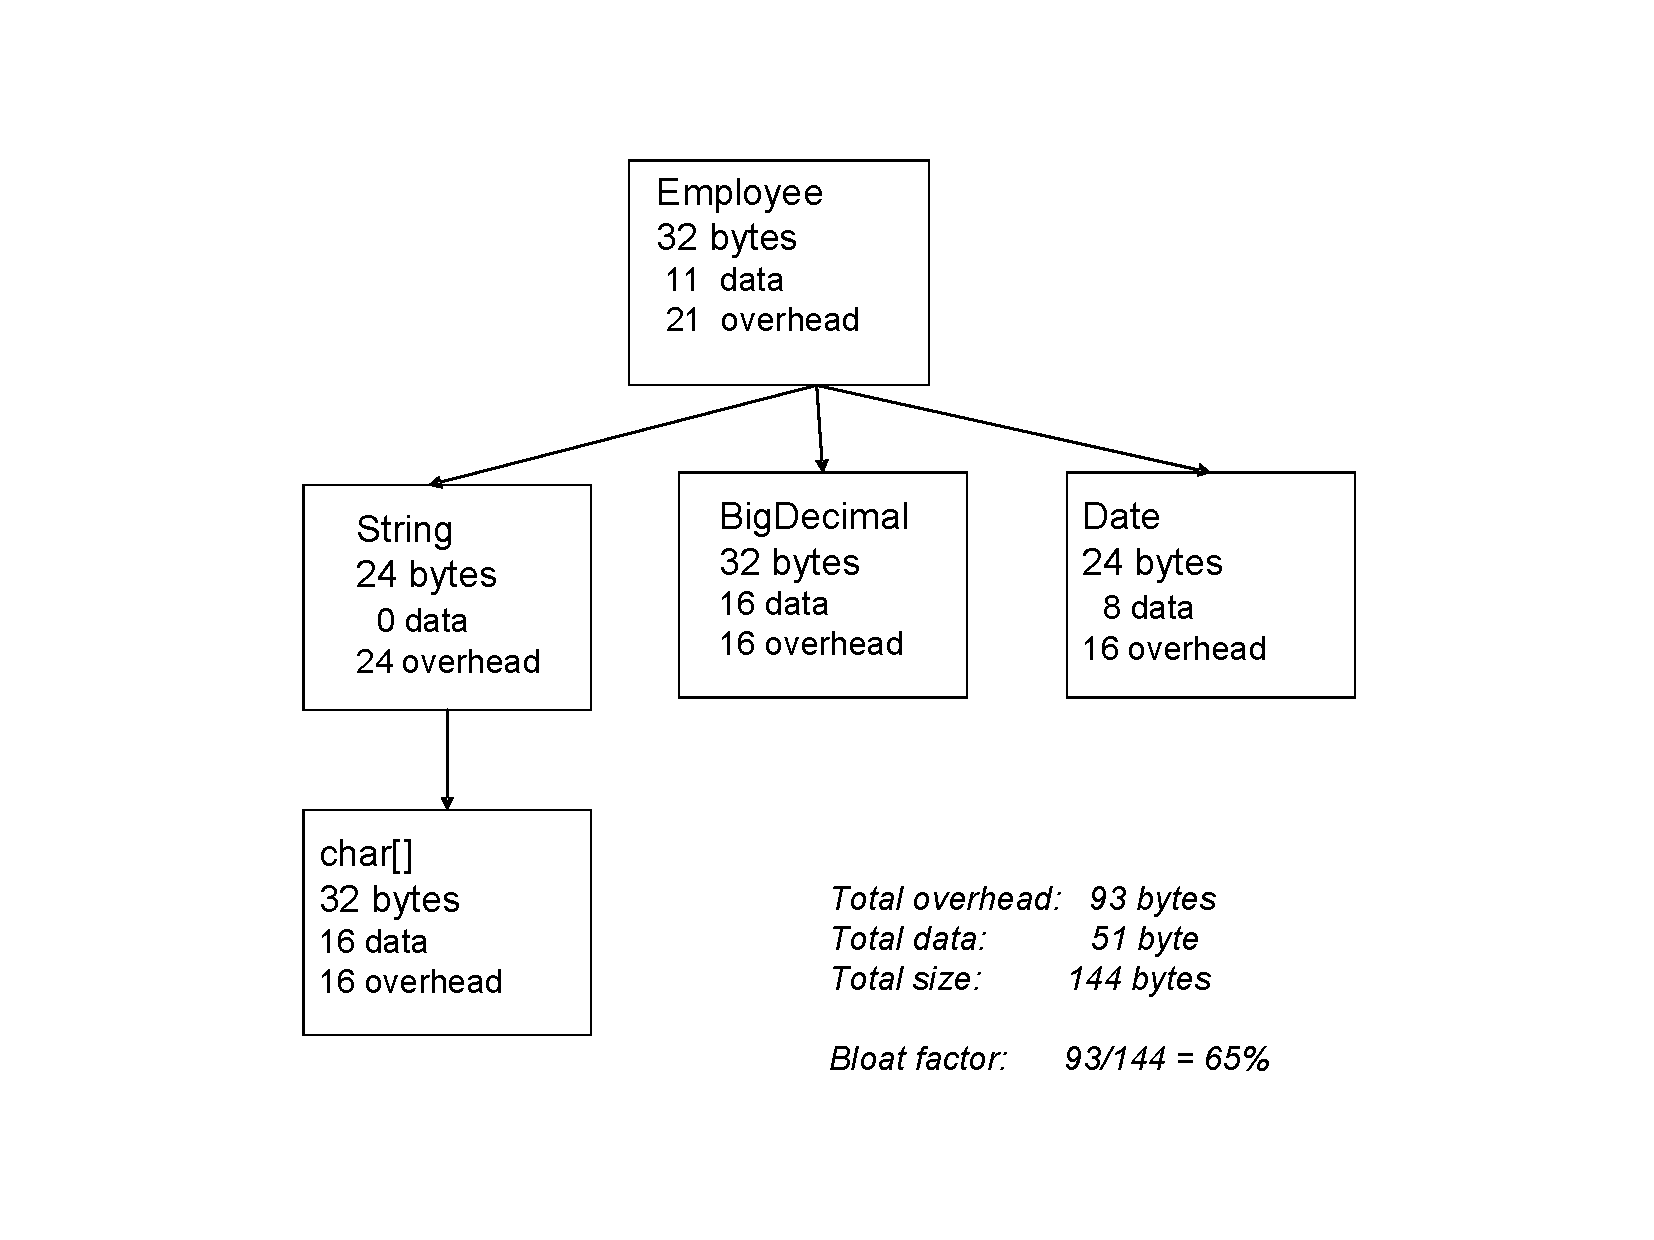
\includegraphics[width=.60\textwidth]{Figures/chapter4/employee-status.pdf}
 % 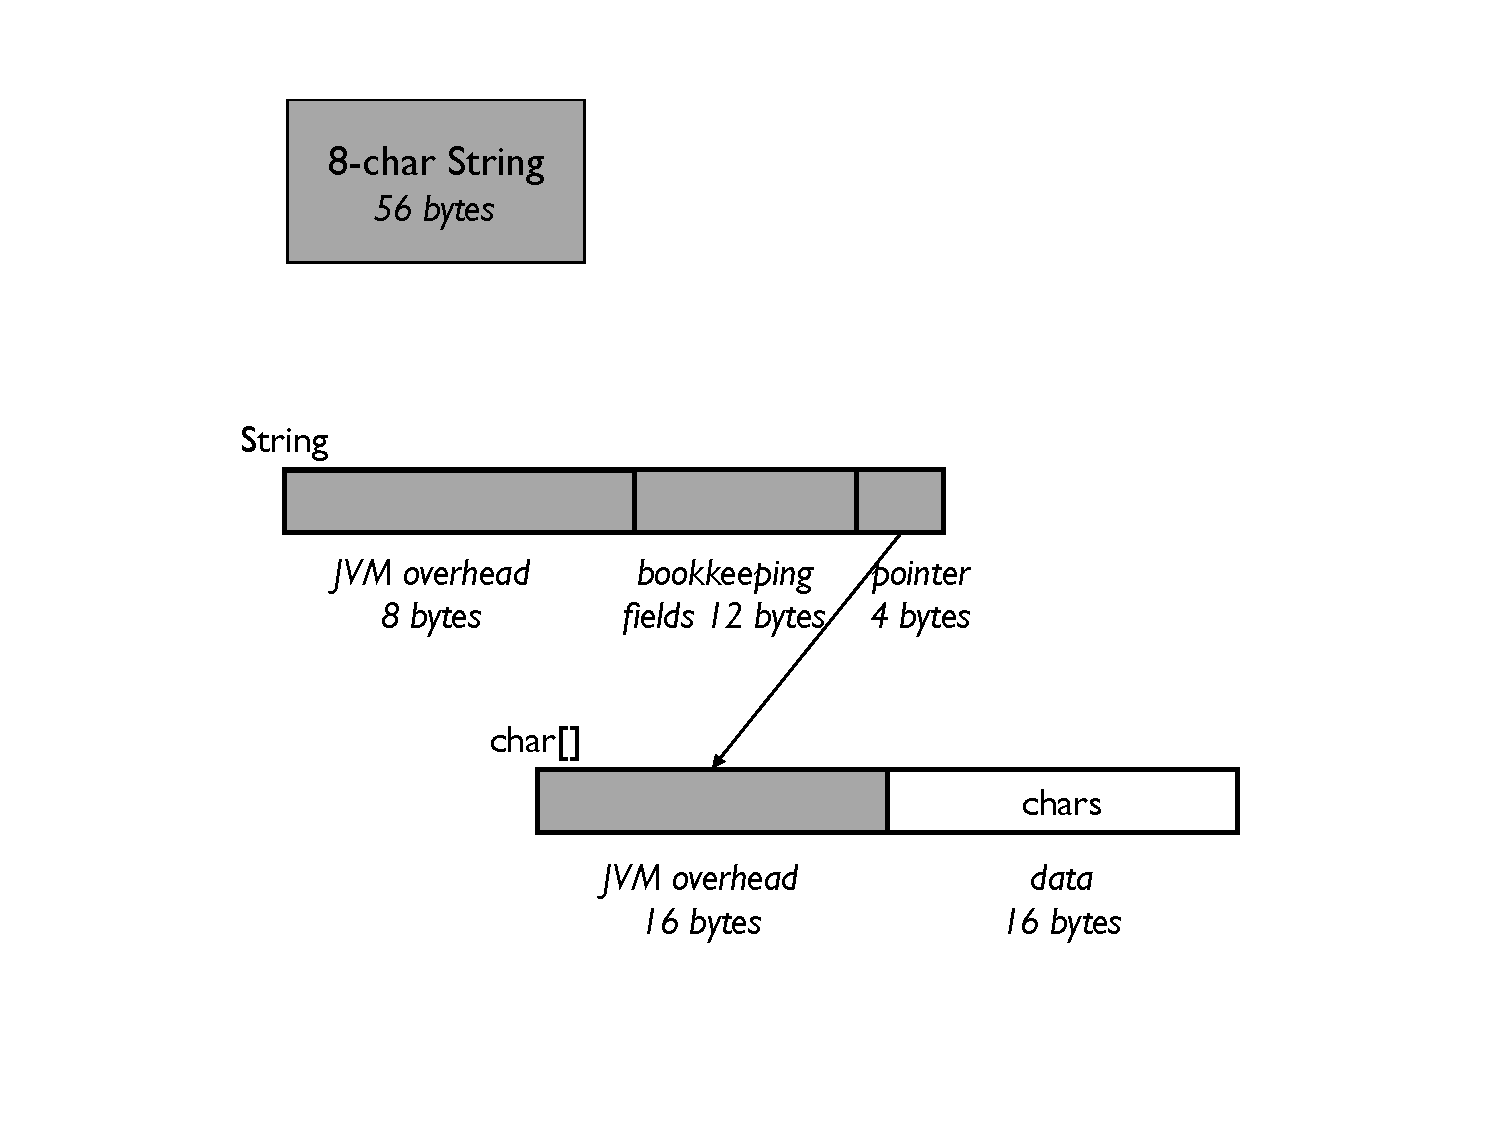
\includegraphics{eight-char-string}
  \caption{The memory layout for an employee "John Doe"}
  \label{fig:employee-status}
\end{figure}

If you compare the total size of 144 bytes with the original \texttt{EmployeeStatus} object size in Section~\cite{CostOfObects}, the storage has more than quadrupled. There are 51 bytes of real data, and 93 bytes of overhead. The bloat factor is now 65\%. As this example shows, delegation increases memory bloat because there is an additional object header and pointer for each delegated object. In this example, there are four delegated objects, so the overhead from delegation alone is 48 bytes. This is 33\% of the total memory cost. Delegation may also force additional alignment costs, since there is another object that has to be aligned to an 8-byte boundary. 
\callout{callout:object-size-estimation-rule}{Delegation Cost Estimation}{
    Every delegation requires an additional pointer in the delegating object and an object header in the delegated object. Therefore, the cost of delegation can be estimated as the cost of an object header plus the cost of a pointer. On 32-bit architectures, a pointer is 4 bytes. This is an estimation because it does not count any extra alignment cost, and the pointer may be null.   
}

Besides delegation, what else contributes to the overhead in Figure ?? ?  First, the entire \texttt{String} object is overhead. Recall from Section\~ref{sec:MemoryBloatFactor} that a \textbf{String} is two objects, a wrapper and a \texttt{char} array, and only the \texttt{char} array has actual data in it.  Secondly, there are some null pointer fields, and alignment bytes. Finally, object header of \texttt{EmployeeStatus} also contributes to the overhead.


In the spirit of keeping things simple, Java does not allow you to nest objects inside other objects. You cannot compose a single object out of other objects, you cannot nest an array inside an object, and you cannot store objects directly in an array.  You can only point to other objects. Even the basic data type \texttt{String} consists of two objects. This means that delegation is pervasive in Java programs, and it is difficult to avoid a high level of delegation overhead. Single inheritance is the only language feature that can be used instead of delegation to compose two object, but single inheritance has limited flexibility.  In contrast, C++ has many different ways to compose objects. C++ has single and multiple inheritance, union types, and variation. C++ allows you to have \texttt{struct} fields, you can put arrays inside of structs, and you can also have an array of structs.  Delegation at this basic level is the price of object oriented programming in Java. This cost is often considered to be insignificant. Delegating to another object is just a single level of indirection. But the costs of the pointers and object headers needed to implement delegation add up quickly, and contribute significantly to large bloat factors in real applications.

\section{64-bit Architectures}

n th 64-bit world, that string is now 96 bytes, and the reason is 50\% larger than it was in 32-bit JVM. The reason is first of all So in this case, just the delegation costs is now 32 bytes, which is basically 1/3 of the cost, and the total cost of the string is up by 50%.  In general, this is a real problem for fine-grained designs. Unfortunately, a lot of designs out there are fine0grained, and we'll see the reasons for that. 


So just lets talk a little about what this means for 64-bit JVMs. People are busting out of this 32-bit address space now, and they are saying let's go to 64-bit, and that will solve everything. Unfortunately, when you go to 64-bit, things blow up pretty quickly. , the object headers are double, pretty sure that's the same thing in sun. arrays are not quite double. 24 bytes. The other thing is that all the pointers instead of being 4 bytes, are now 8 bytes; and finally, there's still that same alignment cost in J9. In SUN you will have a higher alignment cost, since in SUN now it's aligned to 8-byte boundary, where it was aligned to 4-byte boundary before.  The studies I've read, both outside and inside IBM, are showing that going to a 64-bit JVM will increase your memory usage by 40-50\%, and I've heard arguments that say that yur application will run faster, because of the native architecture and all that,  but in some cases there is evidence that it may run slower, because of the worse cache locality. It's another example where it's super important to measure, and not make assumptions that this will fix my speed problem, or it will fix my memory problem. There are a lot of surprises in this area. So J9, and some of the other JVMs, I don't think SUN has this yet, I coud be wrong, I know JRocket has it , they have a mode have called compress addressing, where they can squeeze a few extra bits out of the 32-bit addresses, and in J9 6SR2 is going to allow addressing of up to 28 gig with a 32 bit address still, so without all of these additional footprint problems, if you use this compressing flag. From what I've read, it's only a few percentage degradation in performance, it's pretty minor, so it can certainly help people in this transition area.







\section{Fine-Grained Data Models}
\label{fine-grained-data-models} 

\section{Large Base Classes}

\section{Summary}


\end{document}
